%% Second draft, 17 November 2026: short version (about 25 pages in this layout), in the
%% voice of the MSci thesis. The long first draft is in long/ and feeds supplement.tex.
%% Every number is produced by a script in ../validation (see ../NOTES.md).
%% Lines starting with "%% TODO" are open points for the authors.
\documentclass[preprint,12pt]{elsarticle}

\usepackage{amssymb}
\usepackage{amsmath}
\usepackage{amsthm}
\usepackage{siunitx}
\usepackage{booktabs}
\usepackage{graphicx}
\usepackage[hidelinks]{hyperref}
\renewcommand{\figureautorefname}{Figure}
\renewcommand{\tableautorefname}{Table}
\renewcommand{\sectionautorefname}{Section}
\renewcommand{\subsectionautorefname}{Section}
\usepackage[all]{hypcap}

\graphicspath{{../validation/}{figures/}}

%% let floats share pages with text instead of taking pages of their own
\renewcommand{\topfraction}{0.9}
\renewcommand{\bottomfraction}{0.8}
\renewcommand{\textfraction}{0.08}
\renewcommand{\floatpagefraction}{0.85}
\setcounter{topnumber}{3}
\setcounter{bottomnumber}{2}
\setcounter{totalnumber}{4}

%% table bodies generated by make_tables.py (the primitive \input, so that \bottomrule may follow)
\makeatletter\newcommand{\tablebody}[1]{\@@input tables/#1.tex }\makeatother

\newtheorem{theorem}{Theorem}

%% a smaller bibliography keeps the manuscript near 25 pages
\def\bibfont{\small}

\newcommand{\bE}{\mathbf{E}}
\newcommand{\bH}{\mathbf{H}}
\newcommand{\bG}{\mathbf{G}}
\newcommand{\bx}{\mathbf{x}}
\newcommand{\by}{\mathbf{y}}
\newcommand{\bn}{\mathbf{n}}
\newcommand{\bt}{\mathbf{t}}
\newcommand{\bp}{\mathbf{p}}
\newcommand{\bd}{\mathbf{d}}
\newcommand{\bF}{\mathbf{F}}
\newcommand{\bJ}{\mathbf{J}}
\newcommand{\bK}{\mathbf{K}}
\newcommand{\balpha}{\boldsymbol{\alpha}}
\newcommand{\bbeta}{\boldsymbol{\beta}}
\newcommand{\rhat}{\hat{\mathbf{r}}}
\newcommand{\Einc}{\mathbf{E}^{\mathrm{inc}}}
\newcommand{\sext}{\sigma_{\mathrm{ext}}}
\newcommand{\ssca}{\sigma_{\mathrm{sca}}}
\newcommand{\rmi}{\mathrm{i}}
\newcommand{\rme}{\mathrm{e}}
\newcommand{\supp}[1]{Supplementary Material, Section~S#1}

\journal{Journal of Computational Physics}

\begin{document}

\begin{frontmatter}

%% TODO (authors): title. Alternatives:
%%   "Solving Maxwell's equations with the Method of Fundamental Solutions: edges and tips"
%%   "Where to put the sources: the Method of Fundamental Solutions for Maxwell scattering"
\title{The Method of Fundamental Solutions for Maxwell's Equations on Bodies with Edges}

\author[inst1]{Saptarshi Bandyopadhyay}
\ead{saptarshi.bandyopadhyay.21@ucl.ac.uk}

\author[inst1]{Timo Betcke}
\ead{t.betcke@ucl.ac.uk}

\affiliation[inst1]{organization={Department of Mathematics, University College London},
             addressline={Gower Street},
             city={London},
             postcode={WC1E 6BT},
             country={United Kingdom}}

\begin{abstract}
The Method of Fundamental Solutions (MFS) approximates a scattered field by a sum of point sources placed inside the scatterer. It needs no mesh and converges rapidly for smooth bodies, but its accuracy depends on where the sources are placed, and the usual choice of a scaled copy of the surface fails for bodies with edges or tips. We study the placement of the sources for the scattering of electromagnetic waves by perfect conductors in three dimensions, using four shapes: a sphere, a torus, a cube and the NASA almond. The guiding rule is that the sources must enclose the singularities of the analytic continuation of the field. For the sphere and the torus the sources lie on a smaller copy of the surface, and the error reaches $2\times10^{-14}$ and $7\times10^{-12}$; for the torus we identify a lower bound for the radius of the source surface. For a convex conducting polyhedron we prove that the scattered field is exactly the field of electric and magnetic currents on the interior medial surface of the body, which shows where the sources must go and why both electric and magnetic dipoles are needed. On the cube the sources therefore cluster towards the edges, and below their smallest depth they are continued by a singular tail whose exponents follow from the edge and vertex expansions of the field. Where the usual layout stalls at an error of $21\%$, the error then decays root-exponentially in the number of unknowns down to $1.5\times10^{-5}$, and the field agrees with a boundary element solution to $8\times10^{-5}$. For the almond, sources on the mid-plane with a tail at the tip give a monostatic radar cross-section that agrees with a published reference simulation to $0.14$\,dB or better on average at frequencies up to $10.25$\,GHz.

\end{abstract}

%% The highlights are in highlights.txt (the journal takes them as a separate file).

\begin{keyword}
Method of Fundamental Solutions \sep Maxwell's equations \sep electromagnetic scattering \sep edge singularities \sep method of auxiliary sources \sep radar cross-section
\end{keyword}

\end{frontmatter}

\section{Introduction}
\label{sec:intro}

The method of fundamental solutions (MFS) approximates the solution of a boundary value problem by a sum of point sources placed outside the domain \cite{kupradze1964,fairweather1998}. Each source satisfies the differential equation exactly, so only the boundary condition has to be enforced, at a set of points on the boundary. There is no mesh and no integration. For scattering problems the sources lie inside the scatterer and radiate into the exterior \cite{fairweather2003}. In electromagnetics the same idea is known as the method of auxiliary sources (MAS) or the method of discrete sources \cite{kaklamani2002,doicu2000}.

When the MFS works it converges very quickly. For the Helmholtz equation on analytic domains, Barnett and Betcke \cite{barnett2008} proved exponential convergence for the disc and explained when the method is stable. The solution of the boundary value problem can be continued analytically beyond the boundary, up to a set of singularities. If the sources enclose these singularities, the coefficients stay bounded and the error decays exponentially. If they do not, the coefficients grow exponentially and accuracy is lost in floating-point arithmetic. The MAS literature states the same rule: the auxiliary surface must enclose the singularities of the continued scattered field \cite{leviatan1990,zaridze2002,fikioris2006,tsitsas2018,kyurkchan1996}.

This rule has a consequence that is easy to state. A body with an edge has singularities of the continued field on the edge itself, so no surface inside the body can enclose them. The usual MFS layout, with sources on a shrunk copy of the surface, cannot converge. The MAS literature avoids the difficulty by rounding the edges \cite{bogdanov1999}. In two dimensions the difficulty has been resolved. Lightning solvers place sources in clusters that approach each corner exponentially and reach root-exponential convergence \cite{gopal2019siam,gopal2019pnas}, also for the Helmholtz equation \cite{ginn2023}; Hochman, Leviatan and White \cite{hochman2013} obtained similar layouts earlier by rational fitting. In three dimensions the question is open. Gopal and Trefethen close their paper with the sentence ``The extension to 3D is a bigger issue to be considered'' \cite{gopal2019siam}. Brubeck and Trefethen write that it is ``undoubtedly possible, but not straightforward'' \cite{brubeck2022}. Kong and Shen \cite{kong2026} treat isolated point singularities in three dimensions and call edges and vertices of polyhedra ``particularly challenging''.

For Maxwell's equations the MFS has been used on smooth bodies. Recent examples are the regularised formulation of Ye et al.\ \cite{ye2023} and the solver of Weed et al.\ \cite{weed2026} for layered periodic media, and Kangro \cite{kangro2012} gives a convergence result for analytic surfaces. We are not aware of an MFS for Maxwell scattering that converges on a body with edges or tips.

This paper studies the MFS for the scattering of a plane wave by a perfect electric conductor in three dimensions. It grew out of the first author's MSci thesis \cite{thesis2025}, which applied the MFS to a sphere, a cube and the NASA almond \cite{woo1993}. We keep these shapes and add a torus. The four shapes form a sequence in which the singularities of the continued field move from the centre of the body to its surface:
\begin{itemize}
  \item \emph{Sphere} (\autoref{sec:sphere}). The only singularity is the centre. Dipoles on any inner sphere converge like $\exp(-c\sqrt{N})$ in the number of sources $N$, down to an error of $2\times10^{-14}$ against the Mie series.
  \item \emph{Torus} (\autoref{sec:torus}). The singularities fill a ring inside the tube. Dipoles on an inner torus converge to $7\times 10^{-12}$, provided that its radius exceeds a threshold which we give in closed form.
  \item \emph{Almond} (\autoref{sec:almond}). The singularities lie on a curve in the mid-plane, within 6\% of the rim, and reach the surface at the tip. No inner copy of the surface works. Sources on the mid-plane, clustered towards this curve, do.
  \item \emph{Cube} (\autoref{sec:cube}). The singularities reach the surface along all twelve edges. Sources on the bisector planes of the edges, clustered towards the edges, converge.
\end{itemize}

Our contributions are the following.
\begin{enumerate}
  \item We show that the scattered field of a convex conducting polyhedron is exactly the field of electric and magnetic currents on its interior medial surface (\autoref{thm:skeleton}). This explains where the sources must be placed, why a shrunk surface fails, and why both electric and magnetic dipoles are needed.
  \item We introduce the \emph{singular tail}. Sources that cluster towards an edge or a tip must stop at some smallest distance, and the cut-off limits the accuracy. Below the cut-off we continue the sources, but tie them together with the power laws of the local field expansion, so that they add only a few unknowns. The exponents are not fitted. For an edge they follow from the Meixner expansion \cite{meixner1972}, and for the cube vertex and the almond tip we compute them from the eigenvalues of the Laplace--Beltrami operator outside the corresponding cone \cite{desmedt1986}.
  \item With these layouts the MFS converges on the cube to a relative error of about $10^{-4}$ in the scattered field, and it agrees to $2\times 10^{-4}$ with a boundary element solution on an edge-graded mesh. On the almond the computed monostatic radar cross-section agrees with a published reference simulation \cite{kelley2020} to between 0.01 and 0.14\,dB on average at four frequencies up to 10.25\,GHz.
  \item We compare accuracy against computing time with the boundary element library Bempp \cite{betcke2021} on all four shapes, and we state plainly where the MFS is ahead and where it is not.
\end{enumerate}

\autoref{sec:formulation} states the problem and the method. \autoref{sec:skeleton} explains why inner surfaces fail for the cube and the almond. \autoref{sec:discussion} lists the limits of what we have shown.

\section{The MFS for Maxwell's equations}
\label{sec:method}

\subsection{The scattering problem}

We consider the computation of the electromagnetic field in the unbounded region exterior to a perfect electric conductor (PEC). Here, the conductor occupies a bounded domain $\Omega\subset\mathbb{R}^3$ with surface $\Gamma$, and we work in the frequency domain with time dependence $\rme^{-\rmi\omega t}$ and wavenumber $k$. The incident field is the plane wave
\begin{equation}
  \Einc(\bx) = \bp\,\rme^{\rmi k\,\bd\cdot\bx},
  \label{eq:planewave}
\end{equation}
where $\bp$ is the polarisation vector and $\bd$ the propagation direction. Note that $\bp$ and $\bd$ are orthogonal unit vectors, which is essential for electromagnetic waves in free space. The scattered field $\bE$ satisfies \cite{kirsch2015,colton2013}
\begin{equation}
  \nabla\times\nabla\times\bE - k^2\,\bE = 0 \quad\text{in } \mathbb{R}^3\setminus\overline{\Omega},
  \label{eq:maxwell}
\end{equation}
together with the Silver--M\"uller radiation condition $\lim_{r\to\infty} r\bigl((\nabla\times\bE)\times\hat\bx - \rmi k\,\bE\bigr) = 0$, where $r = \|\bx\|$ and $\hat\bx = \bx/r$, which selects outgoing waves at infinity. On a perfect conductor, the physical requirement is that the tangential component of the total electric field vanishes on $\Gamma$,
\begin{equation}
  \bt\cdot\bigl(\bE + \Einc\bigr) = 0 \quad\text{on } \Gamma
  \label{eq:pec}
\end{equation}
for every tangent vector $\bt$. Equivalently, the currents induced on the surface produce a scattered field that exactly cancels the tangential component of the incident field. Far from the body, the scattered field behaves as an outgoing spherical wave, $\bE(\bx) = \rme^{\rmi kr}\,\bF(\hat\bx)/r + O(r^{-2})$, where $\bF(\hat\bx)$ is the far-field pattern, and the radar cross-section in the observation direction $\hat\bx$ is $4\pi|\bF(\hat\bx)|^2$.

\subsection{The fundamental solution}

Let $\Phi(r) = \rme^{\rmi kr}/(4\pi r)$ with $r = \|\bx-\by\|$ be the outgoing fundamental solution of the scalar Helmholtz equation $(\Delta + k^2)\Phi = -\delta(\bx-\by)$. To lift this scalar solution to a divergence-free vector solution of \eqref{eq:maxwell} away from $\by$, we follow \cite{osipov2017} and apply the operator $I + k^{-2}\nabla\nabla$, since $\nabla\times(\nabla\nabla\Phi\,\balpha) = 0$ and $\Delta\Phi = -k^2\Phi$ for $\bx\ne\by$. Here, $I$ is the unit dyadic, which acts as the $3\times3$ identity on vectors, and $\nabla\nabla\Phi$ is the Hessian of $\Phi$, the $3\times3$ matrix of its second partial derivatives. Writing $\rhat = (\bx-\by)/r$ and noting that the outer product $\rhat\rhat^{\top}$ projects onto the radial direction, we obtain
\begin{equation}
\begin{split}
  \bG(\bx,\by) &= \Bigl(I + \frac{1}{k^2}\nabla\nabla\Bigr)\Phi(r)\\
  &= \Phi(r)\Biggl(\Bigl(1+\frac{\rmi}{kr}-\frac{1}{(kr)^2}\Bigr)I-\Bigl(1+\frac{3\rmi}{kr}-\frac{3}{(kr)^2}\Bigr)\rhat\rhat^{\top}\Biggr).
\end{split}
  \label{eq:dyadic}
\end{equation}
Because this Green's function is a $3\times3$ matrix that connects vector sources to vector fields, it is often referred to as the \emph{dyadic Green's function}. For a vector $\balpha\in\mathbb{C}^3$, the field $\bG(\bx,\by)\,\balpha$ is that of an electric dipole at $\by$ with moment $\balpha$; this field satisfies both \eqref{eq:maxwell} away from $\by$ and the radiation condition. Taking $(1/k)\nabla_{\bx}\times(\bG(\bx,\by)\,\bbeta)$ eliminates the Hessian term and gives a second family of electric-field solutions, radiated by magnetic dipoles at $\by$ with moment $\bbeta\in\mathbb{C}^3$,
\begin{equation}
  \frac{1}{k}\,\nabla_{\bx}\Phi(r)\times\bbeta
  = \Bigl(\rmi-\frac{1}{kr}\Bigr)\Phi(r)\;\rhat\times\bbeta .
  \label{eq:magnetic}
\end{equation}
For the smooth bodies of \autoref{sec:smooth} the electric dipoles are sufficient, whereas bodies with edges need both families, for reasons given in \autoref{sec:skeleton}.

\subsection{Formulation}

We choose $N$ source points $\by_1,\dots,\by_N$ inside the conductor and approximate the scattered field by
\begin{equation}
  \bE_N(\bx) = \sum_{j=1}^{N}\Bigl[\bG(\bx,\by_j)\,\balpha_j + \frac{1}{k}\nabla_{\bx}\Phi(\|\bx-\by_j\|)\times\bbeta_j\Bigr],
  \label{eq:mfs}
\end{equation}
where each coefficient $\balpha_j$ or $\bbeta_j$ is a 3-component vector. As usual, the formulation can be simplified in the implementation by absorbing the constant factor $1/(4\pi)$ of $\Phi$ into the coefficients $\balpha_j$ and $\bbeta_j$, and the coefficient norms reported below follow this convention. Since the approximation satisfies \eqref{eq:maxwell} and the radiation condition for any choice of the coefficients, only the boundary condition \eqref{eq:pec} has to be enforced. We do this at $M$ boundary points $\bx_1,\dots,\bx_M$ on $\Gamma$. At each boundary point an orthonormal tangent basis $\bt_i^{1},\bt_i^{2}$ is computed, and the coefficients are chosen to minimise
\begin{equation}
  \sum_{i=1}^{M} w_i \sum_{s=1}^{2}\bigl|\bt_i^{s}\cdot\bigl(\bE_N(\bx_i)+\Einc(\bx_i)\bigr)\bigr|^2,
  \label{eq:leastsquares}
\end{equation}
where the weight $w_i$ is the surface area that the point represents (modified near the edges of the cube, \autoref{sec:cubepoints}). Since each coefficient is a vector and each dipole field is given by a $3\times3$ matrix, the resulting system is not a simple scalar one: it is composed of $3\times3$ blocks, one for each pair of a boundary point and a dipole, and after projection onto the tangent plane each block is reduced to a $2\times3$ block. Scaling the two rows at $\bx_i$ by $\sqrt{w_i}$ turns \eqref{eq:leastsquares} into a linear least-squares problem $\|A\balpha - \mathbf{b}\|_2$ with $2M$ equations and $3N$ unknowns for electric dipoles (or $6N$ when magnetic dipoles are included). We always take more equations than unknowns, so that the boundary condition is also controlled between the boundary points.

A well-documented disadvantage of the MFS is that this system of equations is often ill-conditioned \cite{fairweather1998,barnett2008}. For the sphere and the torus we therefore solve it with orthogonal factorisations \cite{golub2013}: QR for the sphere, and the singular value decomposition for the small systems of the torus. For the layouts of the cube and the almond, in contrast, the matrices are well conditioned once their columns are scaled to unit norm, with condition numbers below $10^{6}$ in almost all cases (the exception is the cube at three wavelengths for $J\ge9$, where the QR fallback below is used). Because squaring a condition number below $10^{6}$ keeps $\operatorname{cond}(A^{*}A)$ safely within double precision, in these cases we solve the normal equations $A^{*}A\mathbf{c} = A^{*}\mathbf{b}$ via a Cholesky factorisation $A^{*}A = R^{*}R$ and apply two steps of iterative refinement, $\mathbf{c}\leftarrow\mathbf{c} + (R^{*}R)^{-1}A^{*}(\mathbf{b}-A\mathbf{c})$, following the corrected semi-normal equations of Bj\"orck \cite{bjorck1987}. This costs about half as much as QR, and the fields of the cube agree with those of a QR solve to $10^{-13}$. If the Cholesky factorisation finds the matrix too ill-conditioned, the solver falls back to QR. In all cases the cost is $O(MN^2)$ operations, and the systems have at most a few thousand unknowns once the symmetry of the body has been used.

\subsection{Measuring the error}
\label{sec:errors}

For the sphere, the Mie series \cite{mie1908,bohren1998} gives the exact scattered field, and we report the relative error
\begin{equation}
  \varepsilon = \Bigl(\sum\nolimits_{l}|\bE_N(\mathbf{z}_l)-\bE(\mathbf{z}_l)|^2\Bigr)^{1/2}\Big/\Bigl(\sum\nolimits_{l}|\bE(\mathbf{z}_l)|^2\Bigr)^{1/2}
  \label{eq:fielderror}
\end{equation}
at points $\mathbf{z}_l$ on a sphere that encloses the body: $400$ points on the sphere of radius $2$ for the unit sphere and the unit cube ($1500$ points at radius $1.5$ in \autoref{fig:sphere}), $200$ points on the sphere of radius $2.5$ for the torus, and $400$ points on the sphere of radius $0.3$\,m for the almond. For the non-spherical shapes no closed-form solution exists, so we evaluate \eqref{eq:fielderror} with a reference field in place of $\bE$, always stating which. We also report the boundary residual, computed as the square root of \eqref{eq:leastsquares} relative to its value for $\Einc$ alone on the cube and the almond, and as the corresponding root-mean-square tangential residual at $1500$ test points on $\Gamma$ for the sphere and the torus.

We also use two further checks. The first is the optical theorem. Since a perfect conductor absorbs no energy, the total power removed from the incident wave (determined from the forward amplitude $\bF(\bd)$, with $\bar\bp$ the complex conjugate of $\bp$) equals the total power scattered over the unit sphere $S^2$, so the extinction and scattering cross-sections
\begin{equation}
  \sext = \frac{4\pi}{k}\,\operatorname{Im}\bigl(\bar\bp\cdot\bF(\bd)\bigr), \qquad
  \ssca = \int_{S^2}|\bF(\hat\bx)|^2\,\mathrm{d}s(\hat\bx)
  \label{eq:optical}
\end{equation}
are equal for the exact solution. We evaluate $\ssca$ with a Gauss--Legendre rule in the cosine of the polar angle and the trapezoidal rule in the azimuth ($40\times80$ points, or $48\times96$ on the torus and the almond). The quantity $|\sext-\ssca|/\ssca$, referred to below as the optical mismatch, is then a reference-free error indicator. Note, however, that it is not a bound, as an example in \autoref{sec:cubepoints} shows.

The second check is an independent solver. We use the boundary element library Bempp-cl \cite{betcke2021,scroggs2017}, which discretises the surface current in the electric field integral equation with lowest-order divergence-conforming Rao--Wilton--Glisson (RWG) elements \cite{rao1982} on a triangular mesh. It serves both as a reference and as a yardstick for the computing time, and its settings are given in \ref{app:bempp}. All timings in this paper were measured on one machine, with two cores of an Intel Xeon Platinum 8481C processor at $2.2$\,GHz and $8$\,GB of memory, and they include assembly, solution and the evaluation of the field.

\section{Smooth conductors: the sphere and the torus}
\label{sec:smooth}

\subsection{The sphere}

We begin with the familiar domain of the unit sphere, for which the Mie series provides the exact scattered field. The polarisation vector is $\bp = (0,1,0)^\top$ and the propagation direction is $\bd = (0,0,-1)^\top$, so that the plane wave impinges from the positive $z$-axis. We use this wave for all shapes unless stated otherwise. The wavenumber is $k = 2\pi$, so the sphere is two wavelengths across.

Source points are placed on a sphere of radius $R<1$ inside the conductor, while boundary points are distributed on the unit sphere. Both sets are Fibonacci lattices, with $N$ electric dipoles and $M = 2N$ boundary points of equal weight, which gives $4N$ equations for $3N$ unknowns. \autoref{fig:sphere} shows the error against the Mie series. For $R = 0.5$ the error is $2.7\times10^{-3}$ with $N = 100$ sources, $2.0\times10^{-9}$ with $N = 400$ and $2.3\times10^{-14}$ with $N = 1200$. Plotted against $\sqrt{N}$ the curves are straight lines, so the error behaves like $\exp(-c\sqrt{N})$. This is the rate that Kangro proves for analytic surfaces \cite{kangro2012}, and it is the natural one in three dimensions: $N$ points on a sphere resolve spherical harmonics up to a degree proportional to $\sqrt{N}$.

The scattered field of the sphere continues analytically up to the centre, so every radius $R$ encloses the singularity and every radius converges. The rate, however, depends on $R$. A smaller radius converges faster, but the norm of the coefficient vector grows as $R$ decreases, from order one at $R = 0.9$ to above $10^{9}$ at $R = 0.1$ for $N = 400$. Large coefficients of alternating sign cancel in the sum \eqref{eq:mfs}, and the digits lost in the cancellation limit the accuracy: for $R = 0.3$ the error stalls at $2\times10^{-12}$. This is the behaviour known from the scalar Helmholtz equation \cite{barnett2008,thesis2025}. We use $R = 0.5$, which is close to the best choice and keeps the coefficients of order ten or less.

\begin{figure}[htbp]
  \centering
  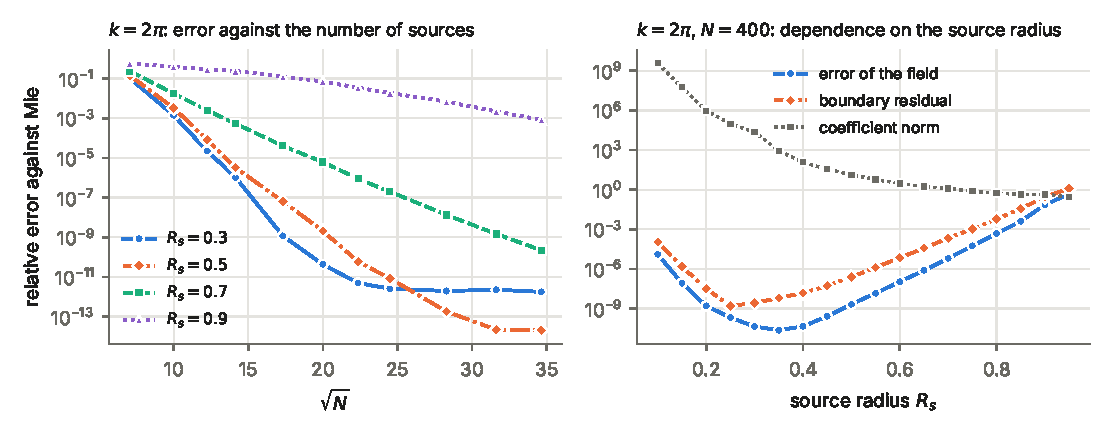
\includegraphics[width=0.95\textwidth]{fig_sphere_short.pdf}
  \caption{MFS for the perfectly conducting unit sphere at $k = 2\pi$, error against the Mie series. Left: error against $\sqrt{N}$ for four source radii $R$. Right: error, boundary residual and coefficient norm against $R$ for $N = 400$.}
  \label{fig:sphere}
\end{figure}

\subsection{The torus}
\label{sec:torus}

The sphere is forgiving because its only singularity is a point. Our second smooth body is the torus $(\rho - R)^2 + z^2 = a^2$, $\rho = \sqrt{x^2+y^2}$, with major radius $R = 1$ and minor radius $a = 0.5$, again at $k = 2\pi$. It is not convex and has no closed-form solution.

The sources are electric dipoles on an inner torus with the same centre circle and minor radius $a_s < a$, arranged on $n_s$ rings around the tube with $n_\varphi$ equally spaced dipoles per ring. The boundary points lie on $2n_s$ rings with $n_\varphi$ points each. Both sets are invariant under rotation by $2\pi/n_\varphi$ about the axis, so the least-squares problem splits exactly into $n_\varphi$ small problems, one for each Fourier mode about the axis, for any incident wave. This is the splitting used by Liu and Barnett for acoustic scattering \cite{liu2016}.

For the torus the admissible source surfaces are bounded from below. Let $c = \sqrt{R^2-a^2}$. The circle $\rho = c$, $z = 0$ is the focal ring of the toroidal coordinates in which the surface is a coordinate surface, and it lies inside the tube, between the centre circle and the inner wall. We find that the continued field is singular on the focal ring, so that a source torus concentric with the tube must satisfy
\begin{equation}
  a_s > R - \sqrt{R^2-a^2}.
  \label{eq:torusradius}
\end{equation}
We have not proved this bound and present it as a conjecture supported by an image argument and two numerical tests (\supp{3}). \autoref{fig:torussources} shows one of the tests. With a fixed number of sources, the norm of the coefficients stays of order one while $a_s$ satisfies \eqref{eq:torusradius} and grows by orders of magnitude below the bound, which is the behaviour that Barnett and Betcke prove for the disc \cite{barnett2008}. We know of no proof in the literature either. Millar's continuation theory for axially symmetric problems \cite{millar1983} assumes a body that meets the axis, and for tori in four and six dimensions the singular set of the related Schwarz potential is the centre circle alone \cite{aberra2002}.

\begin{figure}[htbp]
  \centering
  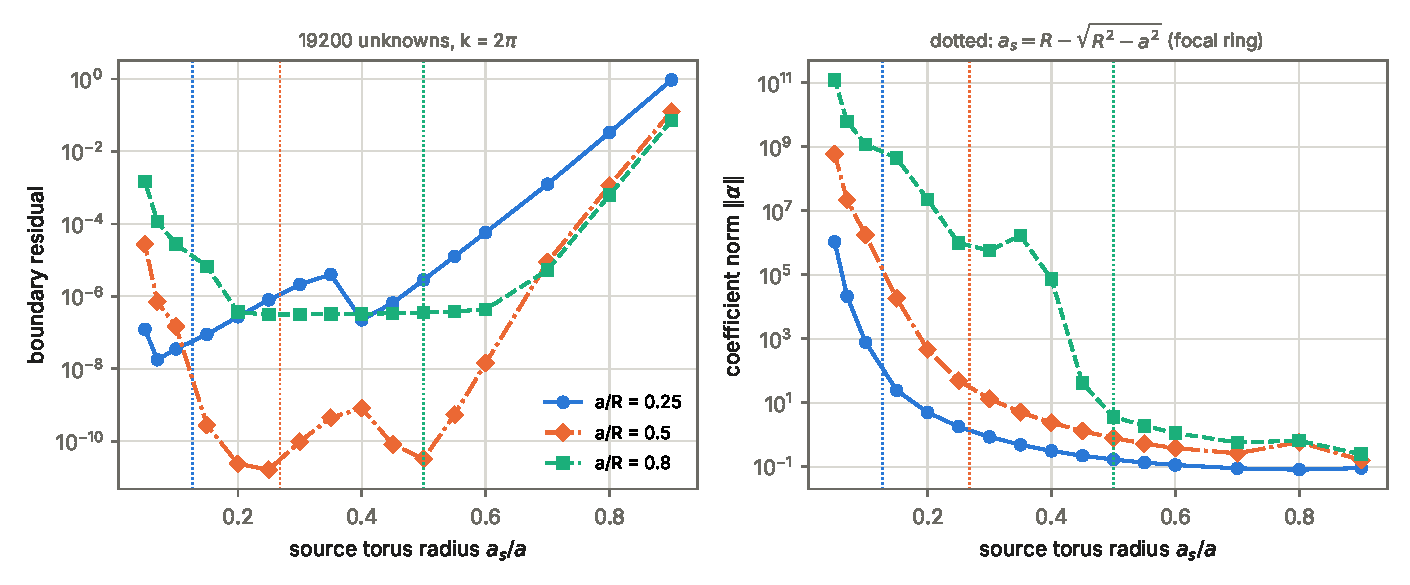
\includegraphics[width=0.85\textwidth]{fig_torus_sources.pdf}
  \caption{Torus with $R = 1$ and three minor radii $a$, $k = 2\pi$, $19200$ unknowns. Boundary residual (left) and coefficient norm (right) against the radius of the source torus. The dotted lines mark the bound \eqref{eq:torusradius}.}
  \label{fig:torussources}
\end{figure}

With $a_s = 0.5\,a$ the error of the scattered field, measured against the finest MFS run, falls from $5.0\times10^{-3}$ with $1440$ unknowns to $7.3\times10^{-12}$ with $21120$ unknowns, and the finest of these runs takes $10$\,s. As an independent check, the extinction cross-section computed by Bempp approaches the MFS value $11.7526$ like the reciprocal of the number of unknowns, and extrapolation gives $11.7533$, a relative difference of less than $10^{-4}$.

\section{Why an inner copy of the surface fails}
\label{sec:skeleton}

The layout of the two previous sections places the sources on a smaller copy of the surface. For the cube and the almond this layout does not converge.

\emph{Cube.} For the unit cube at $k = 2\pi$ we placed between $96$ and $600$ electric dipoles on the faces of a concentric inner cube. The error of the scattered field stays between $21\%$ and $30\%$ and does not decrease as sources are added (\autoref{sec:cube}).

\emph{Almond.} For the NASA almond at $1.19$\,GHz, our first layouts on an inner surface were unstable and failed a test with a known exterior solution. A confocal inner surface that resolves the rim gave a stable fit, but its boundary residual remained at $22\%$ with $1243$ sources.

Both failures have the same cause, and it is the rule quoted in the introduction: the sources must enclose the singularities of the continued field. We now locate these singularities for both shapes.

\subsection{Convex polyhedra}

For a polyhedron the continuation can be written down explicitly. Let $\Omega$ be a convex polyhedron. For each face $F$ let $C_F$ be the set of points of $\Omega$ that are closer to the plane of $F$ than to the plane of any other face. The cells $C_F$ fill $\Omega$, and their common walls form the interior medial surface $\mathcal{M}$ of the polyhedron, which we call its \emph{skeleton}. For the cube the skeleton consists of twelve triangles. Each triangle joins an edge to the centre and lies in the plane that bisects the two faces meeting at that edge.

\begin{theorem}
\label{thm:skeleton}
Let $\Omega$ be a convex perfectly conducting polyhedron with skeleton $\mathcal{M}$, and let $\Einc$ be an entire solution of Maxwell's equations. Then the scattered field outside $\Omega$ is the field radiated by an electric surface current $\bJ$ and a magnetic surface current $\bK$ on $\mathcal{M}$.
\end{theorem}

\begin{proof}
Let $(\bE^{t},\bH^{t})$ be the total field outside $\Omega$. Fix a face $F$ with unit normal $\bn$, let $\bx^*$ be the mirror image of $\bx$ in the plane of $F$, and let $P = I - 2\bn\bn^{\top}$. The reflected field
\begin{equation}
  \bE_F(\bx) = -P\,\bE^{t}(\bx^*), \qquad \bH_F(\bx) = P\,\bH^{t}(\bx^*)
\end{equation}
solves Maxwell's equations wherever $\bx^*$ lies outside $\Omega$. Since $\Omega$ is convex, its mirror image lies outside $\Omega$, so $(\bE_F,\bH_F)$ is defined in all of $\Omega$. On $F$ the total field satisfies $\bn\times\bE^{t} = 0$ and therefore $\bn\cdot\bH^{t} = 0$. Hence the reflected field has the same tangential traces on $F$ as the total field, and it continues the total field analytically across the open face. This is the image principle read backwards.

Define $\mathbf{V} = \bE^{t}$ outside $\Omega$ and $\mathbf{V} = \bE_F$ in each cell $C_F$. Then $\mathbf{V}$ solves Maxwell's equations away from $\mathcal{M}$, and $\mathbf{U} = \mathbf{V} - \Einc$ equals the scattered field outside $\Omega$ and satisfies the radiation condition. We apply the Stratton--Chu representation formula \cite{colton2013} to $\mathbf{U}$ on the two sides of $\mathcal{M}$. Small tubes around the edges and small balls around the vertices contribute nothing in the limit, because the field grows at most like $\rho^{-1/3}$ at distance $\rho$ from an edge and like $r^{\nu-1}$ with $\nu > 0$ at distance $r$ from a vertex \cite{meixner1972,costabel2000}, and the reflected fields inherit the same growth. What remains is the field of the currents
\begin{equation}
  \bJ = \bn_{\mathcal{M}}\times[\bH], \qquad \bK = -\bn_{\mathcal{M}}\times[\bE]
  \label{eq:jumps}
\end{equation}
on $\mathcal{M}$, where $[\,\cdot\,]$ denotes the jump between the continuations from the two neighbouring cells.
\end{proof}

The theorem has three consequences for the method.
\begin{enumerate}
  \item Sources on the skeleton are sufficient, and nothing closer to the faces is needed.
  \item The skeleton contains the edges. A shrunk copy of the surface does not reach them and cannot represent the field. This is the stall at $21$--$30\%$.
  \item Both currents in \eqref{eq:jumps} are non-zero in general, so both electric and magnetic dipoles are needed. With electric dipoles alone, our edge sources stalled at an error of $5\%$.
\end{enumerate}
The densities $\bJ$ and $\bK$ are smooth on each wall of the skeleton and become singular only towards the edges and vertices. This is where the sources must cluster.

\begin{remark}
The statement has a relative in potential theory. Gustafsson \cite{gustafsson1998} showed that a convex polyhedron of uniform density has the same exterior Newtonian potential as a measure supported on finitely many planes inside it, which reaches the boundary only at edges and corners. \autoref{thm:skeleton} is the corresponding statement for scattering by a conductor. To our knowledge it has not been stated in this form. The proof uses convexity. For a non-convex polyhedron the mirror image of the body can re-enter the body, and the statement does not hold as it stands.
\end{remark}

\subsection{Smooth thin bodies}

For a smooth surface there is no reflection formula, but the location of the singularities is known in simple cases. For an ellipse in two dimensions the continued field is singular at the two foci \cite{millar1971,barnett2008}. Every cross-section of the almond is an ellipse with axis ratio $3:1$, whose foci lie at the fraction $\sqrt{1-1/9}\approx0.943$ of the semi-major axis. We therefore expect the singularities of the continued field of the almond on the curve traced by these foci in the mid-plane. This \emph{focal curve} runs within $6\%$ of the rim. A shrunk copy of the surface that stays outside the focal curve would have to lie within $6\%$ of the rim itself, where it is too close to the surface to be useful.

This is the standard continuation argument applied section by section, and it is not a proof for the three-dimensional body. Our evidence is numerical. Sources on the mid-plane that cluster towards the focal curve converge (\autoref{sec:almond}), and sources on surfaces that leave the focal curve outside do not.

The skeleton of the cube and the mid-plane of the almond play the same role. In both cases the sources are placed on a surface inside the body that the continued field cannot cross, and they cluster towards the part of that surface which touches or approaches the boundary.

\section{The cube}
\label{sec:cube}

In this section we construct sources for the unit cube $[-\tfrac12,\tfrac12]^3$ at $k = 2\pi$, so that the side is one wavelength. By \autoref{thm:skeleton} the sources belong on the twelve bisector planes of the edges, and they must resolve current densities that are singular at the edges and vertices. We describe the layout of the sources, the singular tail that continues them towards the edges, and the boundary points, and then present the results.

\subsection{Sources on the skeleton}
\label{sec:cubelayout}

The layout has three kinds of free sources (\autoref{fig:cubelayout}).

\emph{Base points.} A grid of $n_b\times n_b$ electric dipoles on each face of an inner cube at depth $0.2$ below the faces represents the smooth part of the field. These points stand for the inner part of the skeleton, whose field is smooth outside the inner cube.

\emph{Edge lines.} For each edge we choose depths that decrease geometrically,
\begin{equation}
  d_j = 0.2\,q^{\,j}, \qquad j = 0,1,\dots, \qquad \text{down to } d_J = 0.2\cdot 2^{-J},
  \label{eq:depths}
\end{equation}
and place at each depth a line parallel to the edge, on the bisector plane, at depth $d_j$ below the two faces. We call $J$ the level of the layout. We use two ratios: $q = 1/2$, which gives one line per octave of depth, and $q = 2^{-1/2}$, which gives two.

A lightning solver in two dimensions places one point source at each depth \cite{gopal2019siam}. In three dimensions a row of points at depth $d$ would need about $1/d$ of them, so we let each line carry a continuous dipole density instead. With $t$ the coordinate along the line at depth $d$, the stretched variable
\begin{equation}
  u(t) = \frac{1}{\lambda}\log\frac{\tfrac12+t}{\tfrac12-t}, \qquad \lambda = \log\frac{1-d}{d},
\end{equation}
maps the line to $[-1,1]$ and resolves every scale between $d$ and the length of the edge near both vertices. The density is a vector polynomial in $u$ with $n = n_0 + \lceil 2\log(1/d)\rceil$ Legendre modes, and each line exists twice, once with electric and once with magnetic dipoles. A line at depth $10^{-3}$ thus costs about $25$ modes, where a row of points would need a thousand. On the cube the method is therefore no longer free of integration, but the integrals are one-dimensional, and they are evaluated by a quadrature that shares its nodes between the boundary points (\autoref{app:lines}).

\emph{Vertex points.} On the body diagonal through each vertex we place an electric and a magnetic point dipole at each of the same depths.

\begin{figure}[htbp]
  \centering
  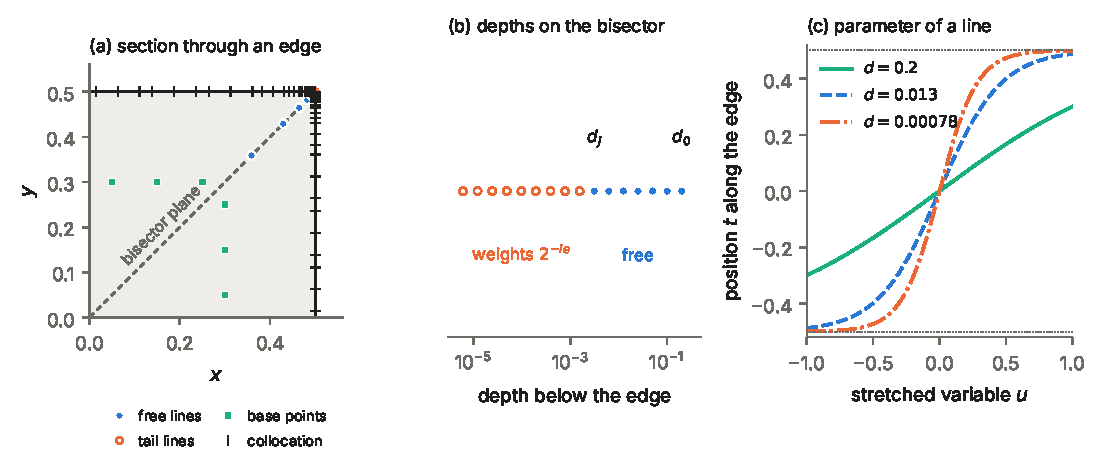
\includegraphics[width=0.8\textwidth]{fig_cube_layout.pdf}
  \caption{Source layout of the cube. (a) Cross-section through the middle of an edge: the lines, seen end on, sit on the bisector plane at the depths \eqref{eq:depths}; base points lie on an inner cube; boundary points on the two faces are graded towards the edge. (b) The depths on a logarithmic scale: free lines down to $d_J$, then the tail with fixed weights. (c) The stretched variable $u$ along a line, which clusters the modes towards the two vertices as the depth decreases.}
  \label{fig:cubelayout}
\end{figure}

\subsection{The singular tail}
\label{sec:tail}

The deepest free line lies at the depth $d_J$. The current sheet of \autoref{thm:skeleton} continues below this depth, all the way to the edge, and cutting it off leaves an error that decays only like $d_J^{0.55}$ in our experiments. To continue the free lines to ever smaller depths would be expensive, and it is not necessary, because close to the edge the form of the currents is known.

We therefore continue the lines at the depths $d_J2^{-i}$, $i = 1,\dots,9$, without new unknowns. These lines are not free: they carry the modes of the line at $d_J$, multiplied by the fixed weights $2^{-ie}$. We call this continuation the \emph{singular tail}. The exponent $e$ is not fitted. It follows from the edge expansion of the field, as we now show.

Consider one edge of the cube, with the coordinate $s$ along the edge and polar coordinates $(\rho,\phi)$ around it, so that the exterior is the wedge $0<\phi<3\pi/2$. Near the edge the field is a sum of terms of two types \cite{meixner1972,costabel2000},
\begin{align}
  E_s &= a_n(s)\,\rho^{2n/3}\sin(2n\phi/3), & n &= 1,2,\dots, \label{eq:tm}\\
  H_s &= b_n(s)\,\rho^{2n/3}\cos(2n\phi/3), & n &= 0,1,2,\dots, \label{eq:te}
\end{align}
each multiplied by a power series in $\rho^2$. The transverse components follow from $E_s$ and $H_s$ and are one power of $\rho$ lower.

The reflection used in the proof of \autoref{thm:skeleton} continues each term into the body by the same formula. The two continuations, through the two faces, meet on the bisector half-plane, which is the wall of the skeleton at this edge. With the angle $\psi = \phi - 3\pi/4$ measured from the exterior bisector, the wall is $\psi = \pi$ seen from one side and $\psi = -\pi$ from the other. The angular factors in \eqref{eq:tm} and \eqref{eq:te} are sines and cosines of $2n\psi/3$. Their jump across the wall is proportional to $\sin(2n\pi/3)$ for the part that is odd in $\psi$ and vanishes for the even part. Terms with $n$ a multiple of three do not jump: they are polynomial fields and need no sources.

Let $m$ be the mirror in the bisector plane. A term is even under $m$ if $E_s$ is even in $\psi$ or $H_s$ is odd in $\psi$. For an even term the tangential electric field is continuous across the wall and the tangential magnetic field jumps, so by \eqref{eq:jumps} it leaves only an electric current. An odd term leaves only a magnetic current. Reading off the leading jumps gives the current densities of \autoref{tab:edgeexp}, where $\rho$ is now the depth on the wall. The electric current behaves like $\rho^{-1/3}$ along the edge and like $\rho^{2/3}$ along the bisector, and the magnetic current like $\rho^{1/3}$ and $\rho^{4/3}$.

It remains to turn the densities into weights. The tail replaces the current sheet below $d_J$ by lines at the depths $d_J2^{-i}$, and a line stands for the strip of the sheet around it, whose width is proportional to its depth. A density $\rho^{e-1}$ therefore gives the line weights $2^{-ie}$, with $e = 2/3$, $5/3$, $4/3$ and $7/3$ for the four components.

\begin{table}[htbp]
  \centering
  \caption{Exponents of the edge tail of the cube. The current density on the bisector half-plane behaves like $\rho^{e-1}$ at depth $\rho$ below the edge.}
  \label{tab:edgeexp}
  \begin{tabular}{llll}
    \toprule
    Current & Component & Density & Tail exponent $e$ \\
    \midrule
    electric, $J_s = [H_\rho]$ & along the edge & $\rho^{-1/3}$ & $2/3$ \\
    electric, $J_\rho = [H_s]$ & along the bisector & $\rho^{2/3}$ & $5/3$ \\
    magnetic, $K_s = [E_\rho]$ & along the edge & $\rho^{1/3}$ & $4/3$ \\
    magnetic, $K_\rho = [E_s]$ & along the bisector & $\rho^{4/3}$ & $7/3$ \\
    \bottomrule
  \end{tabular}
\end{table}

The vertex points are continued in the same way along the diagonal. Near a vertex the field behaves like $r^{\nu-1}$ in the distance $r$, and the tail weights of the electric and magnetic dipoles have the exponents $\nu+2$ and $\tau+2$, where $\nu = 0.4542$ and $\tau = 0.840$ are the smallest electric and magnetic exponents of the corner. We computed them from eigenvalue problems on the sphere (\autoref{app:cone}), and they agree with the values $0.45410$ and $0.84108$ of De Smedt and Van Bladel \cite{desmedt1986}.

The tails are cheap: at $J = 8$ all of them together are $9\%$ of the unknowns. \autoref{fig:edgeresidual} shows their effect on the residual at the boundary. Without the tail the residual is of order one at all distances from the edge below $d_J$. With the tail it stays near $10^{-2}$ or below down to the end of the tail at $d_J2^{-9}$, so the strip in which the boundary condition is violated is narrower by a factor of $2^{9}$.

\begin{figure}[htbp]
  \centering
  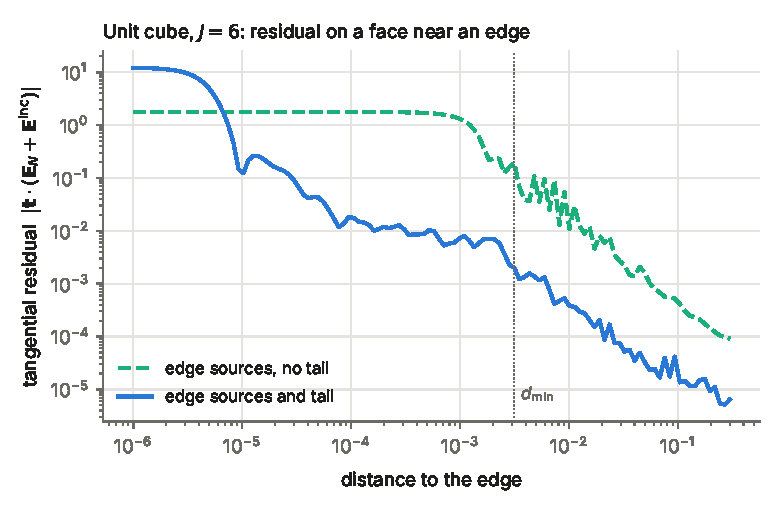
\includegraphics[width=0.6\textwidth]{fig_edge_residual.pdf}
  \caption{Unit cube, $J = 6$, one depth per octave: tangential residual on a face as a function of the distance to an edge, away from the vertices, with and without the tail. The dotted line marks the deepest free depth $d_J$.}
  \label{fig:edgeresidual}
\end{figure}

\subsection{Boundary points, weights and symmetry}

The boundary points on each face form a tensor grid. In each direction the nodes are Gauss--Legendre points on panels that halve in length towards both edges until they are shorter than $d_J$, and panels in the interior are no longer than $h_{\max}$. We use three nodes per panel for $q = 1/2$ and four for $q = 2^{-1/2}$. The fit needs enough equations at every scale: with two nodes per panel and $q = 1/2$ the error at $J = 5$ is $85\%$, although the residual at the boundary points is small.

The rows are weighted by $w_i = A_i\,\rho_i$, where $A_i$ is the area represented by the point and $\rho_i$ its distance to the nearest edge, so that the fit does not spend its effort on the edge singularity of the residual. All resolution parameters grow together with the level: $n_0 = \max(4, 2J-4)$, and $(n_b, h_{\max}) = (4, 0.25)$ for $J\le5$ and $(6, 0.15)$ for $J\ge6$.

The cube and the layout are symmetric under the three mirrors $x\to-x$, $y\to-y$ and $z\to-z$. Any incident field is the sum of eight parts of definite parity, and each part needs only the sources and boundary points of one octant. The eight matrices are signed sums of the same reflected blocks, so the line integrals are computed once, and the factorisation of a class serves every incident wave. Our standard wave excites two classes, and a general wave excites all eight.

\subsection{Results}
\label{sec:cuberesults}

\autoref{tab:cube} lists the results for both depth ratios, and \autoref{fig:cubeconv} shows them against the number of unknowns. Since the cube has no exact solution, the reference is the finest layout, with two depths per octave at level $J = 11$. We first describe the convergence and then the evidence that the limit is the correct field.

\begin{table}[htbp]
  \centering
  \caption{Unit cube, $k = 2\pi$. MFS with edge sources and tails, with one and with two source depths per octave: unknowns and equations per parity class (two classes are solved), wall time, difference from the run with two depths per octave at $J = 11$, and optical mismatch.}
  \label{tab:cube}
  \small
  \begin{tabular}{lrrrrll}
    \toprule
    Depths & $J$ & Unknowns & Equations & Time [s] & Error & Optical \\
    \midrule
\tablebody{cube_mfs_short}
    \bottomrule
  \end{tabular}
\end{table}

With two depths per octave the error falls from $5.1\times10^{-3}$ at $J = 4$ to $1.5\times10^{-5}$ at $J = 10$, by a factor of $2.4$ to $3.5$ per level, and the optical mismatch falls with it to $1.8\times10^{-6}$. Let $N$ be the number of unknowns of the whole cube, which is eight times the entry of \autoref{tab:cube}. Against $\sqrt{N}$ the errors lie on a straight line (\autoref{fig:cubeconv}),
\begin{equation}
  \varepsilon \approx 0.44\,\exp\bigl(-0.048\sqrt{N}\bigr),
  \label{eq:rootexp}
\end{equation}
to within a factor of $1.3$ over two and a half orders of magnitude. This is the root-exponential convergence of the lightning solvers in two dimensions \cite{gopal2019siam}, and it is what the layout suggests: both the number of lines and the number of modes per line grow linearly with the level, and the error decays geometrically with the level. Measured as an algebraic order, the rate rises from about $N^{-2.5}$ to $N^{-6}$ along the table.

\begin{figure}[htbp]
  \centering
  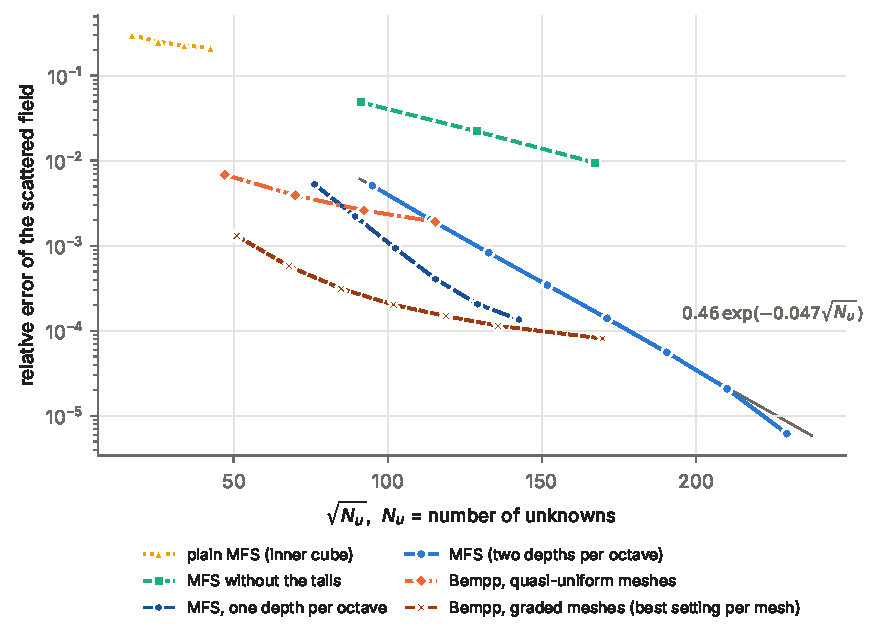
\includegraphics[width=0.78\textwidth]{fig_cube_convergence.pdf}
  \caption{Unit cube, $k = 2\pi$: error of the scattered field against the square root of the number of unknowns $N$ of the whole cube (for the MFS, all eight parity classes together). The grey line is the fit \eqref{eq:rootexp} to the layout with two depths per octave. For Bempp the smallest error over all settings is shown for each mesh.}
  \label{fig:cubeconv}
\end{figure}

The layout with one depth per octave has about $60\%$ of the unknowns and takes between $30\%$ and $60\%$ of the time. Down to level $J = 7$ its errors equal those of the denser layout to within $20\%$, and then it stalls near $1.5\times10^{-4}$. The matrices are well conditioned, so this is not an effect of rounding. The two-dimensional analogue behaves in the same way: for the unit square with point sources on the bisectors of the corners, the error of the far field stalls at $8\times10^{-5}$ for $q = 1/2$, at $6\times10^{-6}$ for $q = 0.6$ and at $10^{-9}$ for $q = 2^{-1/2}$. We therefore regard $q = 1/2$ as the economical choice for errors down to $2\times10^{-4}$ and $q = 2^{-1/2}$ as the choice below.

The tails are essential for this convergence. With the same edge lines but without the tails, the error is $5.4\times10^{-2}$, $2.5\times10^{-2}$ and $1.1\times10^{-2}$ for $J = 4$, $6$ and $8$, so at $J = 8$ the tails reduce the error by a factor of $64$. The exponents matter as well. Adding the next term of each edge expansion to the tail changes the error by less than $1\%$ of its value, but lowering the exponents of the two transverse components by one gives an error of $65\%$.

Three checks support the reference. First, the result is insensitive to the parameters of the layout: at $J = 9$ the field changes by less than $3\times10^{-6}$ when the modes, the tails, the base grid or the boundary grid are refined. Second, a run at $J = 12$ with a finer interior grid ($n_b = 8$, $h_{\max} = 0.1$) differs from the reference by $7\times10^{-6}$ and has an optical mismatch of $9\times10^{-7}$. Third, we computed the same field with Bempp on meshes graded towards the edges. With $10368$, $14112$, $18432$ and $28800$ unknowns the boundary element field differs from the MFS reference by $2.0\times10^{-4}$, $1.5\times10^{-4}$, $1.1\times10^{-4}$ and $8\times10^{-5}$, and its extrapolated extinction cross-section is $2.92786$, where the MFS gives $2.92798$. The two methods thus agree to $8\times10^{-5}$ in the field and to $4\times10^{-5}$ in the cross-section. Below that level the only reference for the MFS is its own convergence.

%%OTHERCASES%%

\section{The NASA almond}
\label{sec:almond}

Our last shape is the NASA almond \cite{woo1993}, a standard test case in computational electromagnetics. It is a smooth body of length $L = 0.2524$\,m with a rounded rear and a sharp tip, whose cross-sections are ellipses with axis ratio $3{:}1$. We place the almond with its long axis along $x$, the tip at positive $x$ and its mid-plane in $z = 0$. It is symmetric under the mirrors $y\to-y$ and $z\to-z$. The almond combines the two difficulties met so far: a singular set close to the surface, as for a thin torus, and a point where it reaches the surface, as at the edges of the cube.

\subsection{Sources on the mid-plane}

By \autoref{sec:focal} the sources lie on the mid-plane and cluster towards the focal curve, which runs at the fraction $\eta_F = 0.943$ of the half-width (\autoref{fig:almondlayout}). They are point dipoles arranged in rows. In the front half a row follows the outline of the mid-plane section at a fixed fraction $\eta$ of the half-width, and in the rear half it continues as the ellipse through the same point of the widest section that is confocal with the focal ellipse. We use $n_{\mathrm{mid}}$ rows in the middle of the section and $n_F+1$ rows at
\begin{equation}
  \eta_j = \eta_F - 2\,(1-\eta_F)\,2^{-j}, \qquad j = 0,\dots,n_F,
\end{equation}
which approach the focal curve geometrically from the inside, and we write $n_{\mathrm{mid}}{:}n_F$ for a layout. The rows in the middle lie at the fractions $\bigl(\eta_F - 3(1-\eta_F)\bigr)\cos\bigl((i+\tfrac12)\pi/(2n_{\mathrm{mid}})\bigr)$, $i = 0,\dots,n_{\mathrm{mid}}-1$. Along a row the spacing of the sources is a fixed multiple of the local distance to the surface, and the boundary points follow the same rule with half that multiple or less, such that there are at least $2.5$ equations for each unknown. Sources and boundary points thus refine together towards the rim.

As for the cube, we use the symmetry. An incident wave is split into its four parts of definite parity under the two mirrors, and each part is solved on one quarter of the body. A source on the mid-plane then keeps three of its six dipole components: the two electric components in the plane and the magnetic component normal to it for the classes that are even under $z\to-z$, and the other three for the odd classes.

\begin{figure}[htbp]
  \centering
  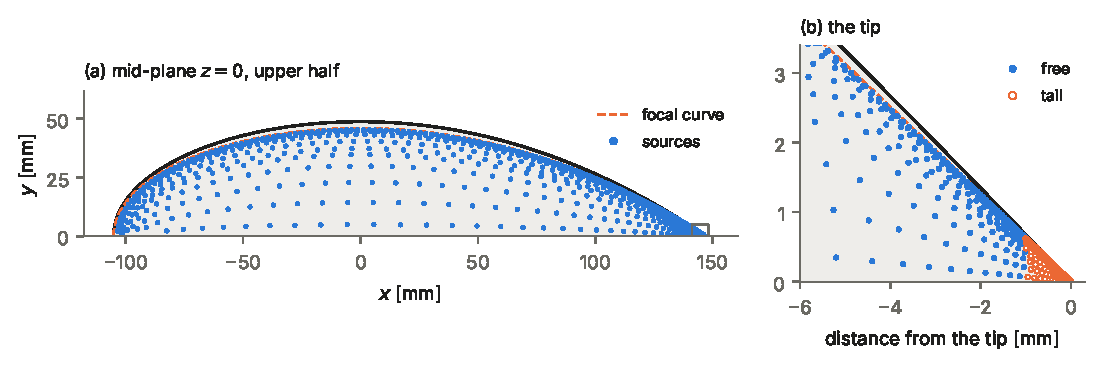
\includegraphics[width=0.8\textwidth]{fig_almond_layout.pdf}
  \caption{Source layout of the almond in the mid-plane $z = 0$ (one half shown). The rows of point dipoles cluster towards the focal curve (dashed), which runs within $6\%$ of the rim, and continue into the tip as a tail.}
  \label{fig:almondlayout}
\end{figure}

\subsection{A tail at the tip}

The focal curve reaches the surface at the tip, which is the vertex of an elliptic cone with half-angles $34.09^\circ$ and $12.71^\circ$. The field of a conducting cone behaves like $r^{\nu-1}$ at distance $r$ from the vertex \cite{desmedt1986}. For this cone we computed the smallest exponent $\nu = 0.2996$ (\ref{app:cone}), so the electric field grows like $r^{-0.70}$ towards the tip.

The free source rows stop $1$\,mm from the tip. The singular term belongs to the parity class that is even under both mirrors, and for this class the cut-off leaves a boundary residual of $19\%$, with a cross-section at oblique angles that is wrong by up to $1.2$\,dB. Adding sources does not help. The remedy is the tail of \autoref{sec:tail}. Each row is continued to within $10^{-4}$\,mm of the tip, and the continued dipoles of a row are tied together with the weights $(r/r_{\mathrm{cut}})^{\nu+2}$ for electric and $(r/r_{\mathrm{cut}})^{\tau+2}$ for magnetic dipoles, where $r_{\mathrm{cut}}$ is the distance of the cut-off from the tip. We use the two smallest electric exponents $\nu$ and the smallest magnetic exponent $\tau$ of the parity class, each with its own coefficient for every row and dipole component, which adds $50$ unknowns per class. For the class that is even under both mirrors these are $\nu = 0.2996$ and $1.464$ and $\tau = 1.975$ (\autoref{tab:coneexp}). With the tail the residual of this class falls from $19\%$ to $0.034\%$.

\subsection{Results}

We first consider the wave that travels along $-x$ and meets the tip first (nose-on incidence), polarised along $y$, at $1.19$\,GHz, where the almond is one wavelength long. Here the sources are spaced along the rows at $0.7$ times their distance to the surface. Measured against the finest layout, $8{:}5$ with $4791$ unknowns, the layouts $5{:}2$ and $6{:}3$, with $2103$ and $2937$ unknowns, differ by $2.8\times10^{-4}$ and $5.6\times10^{-5}$. Refining the reference layout in three different ways changes its field by less than $10^{-5}$.

The quantity of practical interest is the monostatic radar cross-section as a function of the azimuth in the plane of the almond, for the polarisations HH (electric field in the plane) and VV (electric field along $z$). The factorisation of a parity class serves all look angles, so one frequency, with $361$ look angles from $0^\circ$ to $180^\circ$ and both polarisations, takes about two minutes with the layout $6{:}3$. We compare with the Austin RCS Benchmark Suite \cite{kelley2020}, which provides measurements of this almond and a reference simulation with $397{,}674$ unknowns at $3.5$, $5.125$, $7$ and $10.25$\,GHz. At the highest frequency the almond is $8.6$ wavelengths long. We use the same layout $6{:}3$ at all four frequencies, with a closer spacing of the sources along the rows ($0.5$ times the distance to the surface instead of $0.7$), which gives $4193$ unknowns for each of the four parity classes.

\autoref{fig:almondbench} shows the three sets of curves, and \autoref{tab:almondbench} lists the mean absolute difference in decibels over the look angles. The MFS differs from the reference simulation by $0.04$ to $0.14$\,dB for HH and by $0.01$ to $0.02$\,dB for VV. For comparison, the two finest meshes of the reference simulation differ from each other by $0.07$ and $0.02$\,dB at $7$\,GHz \cite{kelley2020}. Both simulations differ from the measurements by $0.6$ to $1.8$\,dB, which is the level at which the measurements are stated to agree with simulation, $\pm1$\,dB for HH and $\pm2$\,dB for VV \cite{kelley2020}.

\begin{table}[htbp]
  \centering
  \caption{NASA almond, monostatic cross-section: mean absolute difference in dB between the MFS (layout $6{:}3$) and the reference simulation of the Austin benchmark \cite{kelley2020}, over $361$ look angles.}
  \label{tab:almondbench}
  \begin{tabular}{lrrrr}
    \toprule
    Frequency [GHz] & 3.5 & 5.125 & 7 & 10.25 \\
    \midrule
    HH & 0.043 & 0.055 & 0.072 & 0.140 \\
    VV & 0.011 & 0.013 & 0.016 & 0.024 \\
    \bottomrule
  \end{tabular}
\end{table}

\begin{figure}[htbp]
  \centering
  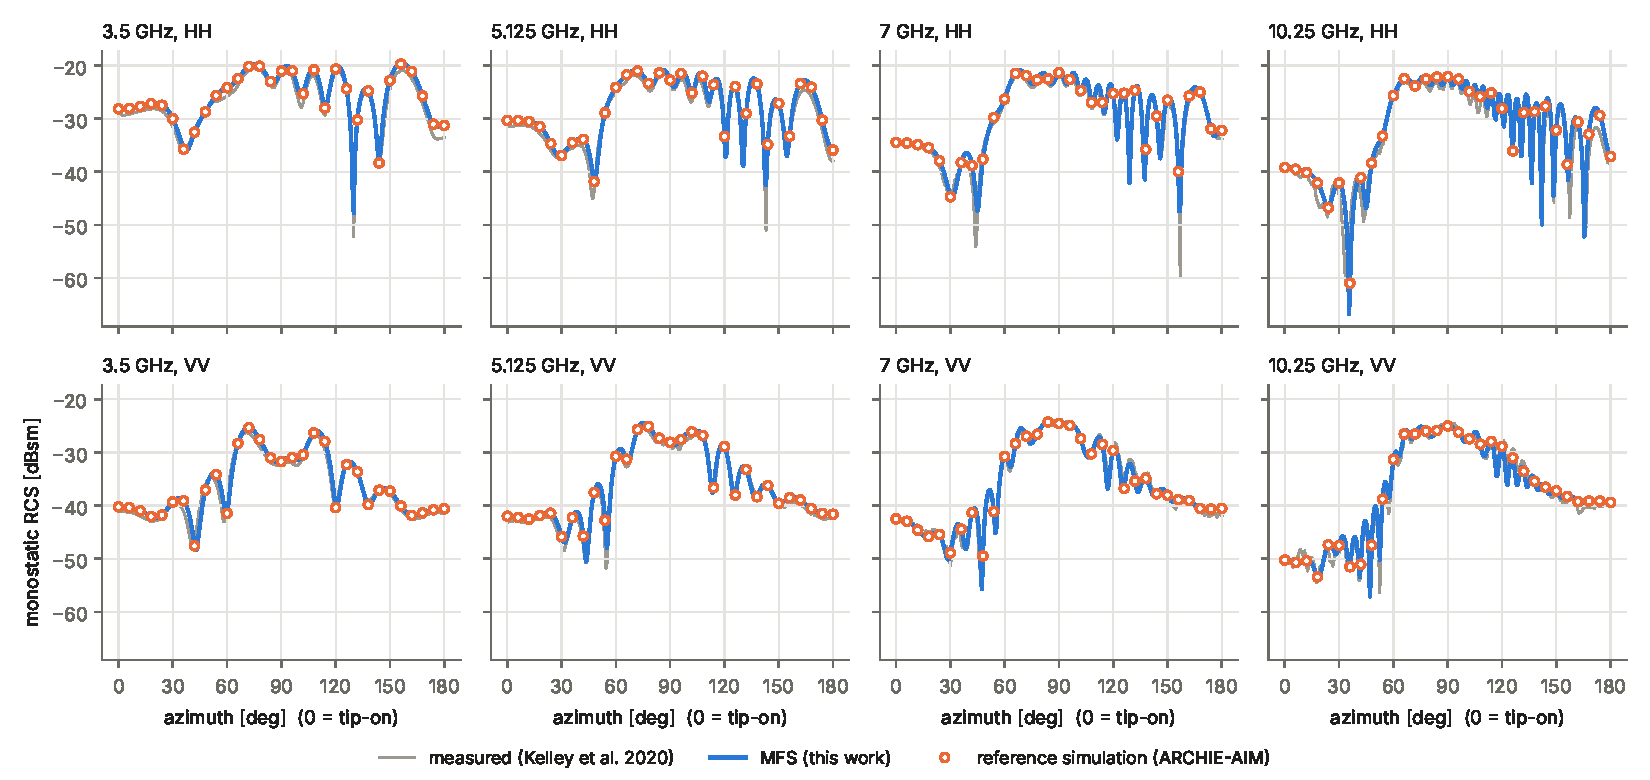
\includegraphics[width=0.9\textwidth]{fig_almond_benchmark.pdf}
  \caption{NASA almond: monostatic radar cross-section against azimuth ($0^\circ$ is nose-on) at four frequencies, HH and VV. MFS, reference simulation and measurements of the Austin benchmark \cite{kelley2020}.}
  \label{fig:almondbench}
\end{figure}

The largest pointwise differences from the reference simulation occur in deep nulls of the HH cross-section, where the reference itself is least certain: its two finest meshes differ by up to $0.5$\,dB near the nulls \cite{kelley2020}. The largest difference is $4.3$\,dB at $10.25$\,GHz and $35.5^\circ$, in a null at $-66.7$\,dBsm. The MFS is converged there, since the layouts $6{:}3$ and $8{:}5$ differ by $0.024$\,dB in this null. The difference is one of position and not of depth: shifting the MFS curve by $0.1^\circ$ halves its distance from the reference samples around this sharp null.

In summary, the MFS agrees with the reference simulation to $0.14$\,dB or better on average. At $7$\,GHz, where the comparison can be made, this is the size of the difference between the two finest meshes of that simulation. The MFS needs four systems of about $4200$ unknowns each where the reference uses $397{,}674$ unknowns. The computing time at the lowest frequency is compared with the boundary element method in the next section.

\section{Comparison with a boundary element code}
\label{sec:cost}

In this section we compare accuracy against wall time for the MFS and the boundary element library Bempp \cite{betcke2021} (\autoref{fig:costall}, \autoref{tab:summary} and \autoref{tab:cubeends}). For exterior scattering in a homogeneous medium by bodies with sharp edges and tips, the weakly singular Galerkin electric-field integral equation (EFIE) is the most direct benchmark: unlike volumetric finite-element or finite-difference schemes, which mesh an artificial exterior box with perfectly matched layers and incur numerical dispersion and truncation reflections, it discretises $\Gamma$ alone and satisfies the radiation condition analytically; and unlike magnetic-field or smooth-surface Nystr\"om integral equations \cite{burbano2026}, it applies directly at sharp wedges and conical vertices \cite{rao1982,bespalov2010}. At these electrical sizes, dense direct factorisation also outperforms unpreconditioned GMRES (which stagnates on edge-graded EFIE matrices) and avoids the sixfold barycentric dual-mesh overhead of Calder\'on preconditioning. To run lowest-order Bempp at its best, we used its OpenCL dense backend, graded the polyhedral meshes towards the edges, scanned gradings, quadrature orders and mesh sizes to form its \emph{lower envelope} (retaining runs at least $3\%$ more accurate than every faster run), and equipped it with the exact mirror, half-turn and rotational symmetries of the MFS (\ref{app:bempp}), speeding Bempp up by three to twenty times without loss of accuracy. Direct comparisons were timed alternately on an idle machine, keeping the minimum time of repeated runs.

\begin{figure}[htbp]
  \centering
  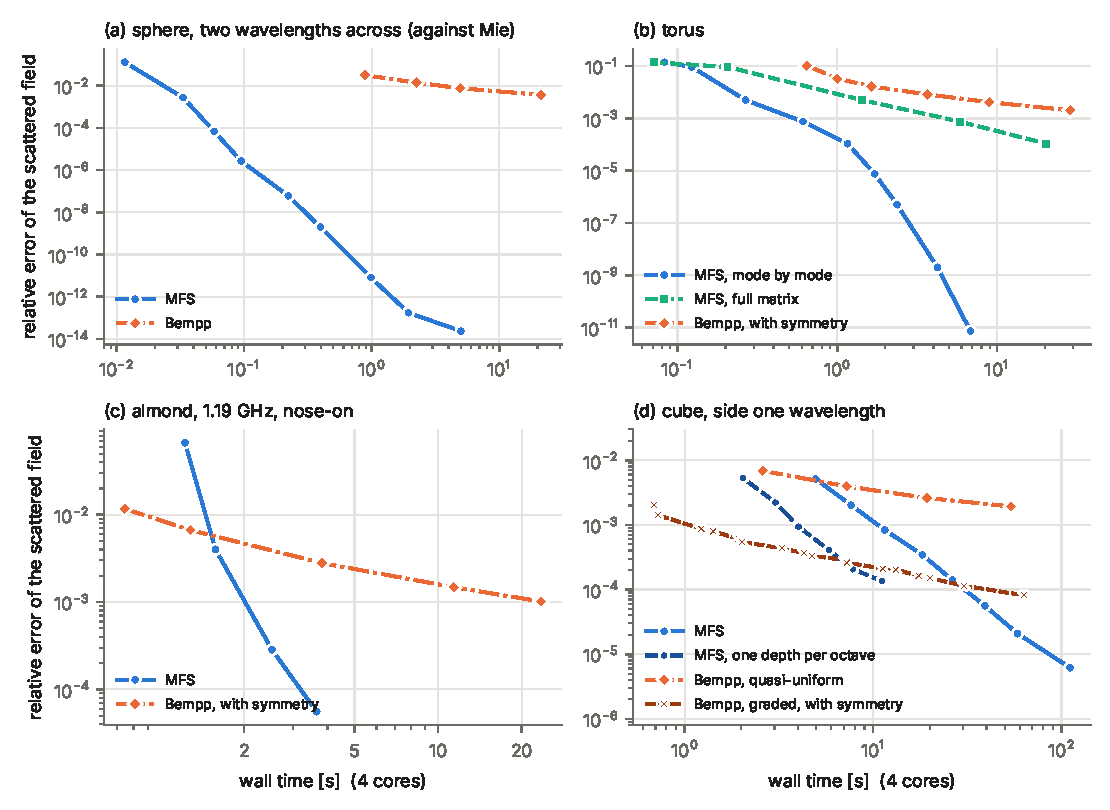
\includegraphics[width=\textwidth]{fig_cost_all.pdf}
  \caption{Error of the scattered field against wall time on two cores for the MFS and for Bempp. (a) Unit sphere at $k = 2\pi$, error against the Mie series. (b) Torus ($R = 1$, $a = 0.5$) at $k = 2\pi$, difference from the finest MFS run; both codes use the rotational symmetry. (c) NASA almond at $1.19$\,GHz, nose-on, difference from the finest MFS layout; both codes use the two mirror planes. (d) Unit cube at $k = 2\pi$, difference from the finest MFS layout (\autoref{sec:cuberesults}): the MFS from $J = 3$ with two depths and one depth per octave (combined lower envelope shaded), Bempp on quasi-uniform meshes, and the lower envelope of symmetric graded Bempp up to its $8$\,GB memory limit.}
  \label{fig:costall}
\end{figure}

\subsection{Smooth bodies and the almond}

On the sphere, the torus and the nose-on almond at $1.19$\,GHz, the MFS reaches errors between $5.6\times10^{-5}$ and $3.5\times10^{-14}$ in ten seconds or less, whereas Bempp's largest meshes reach $2.6\times10^{-4}$ to $2.3\times10^{-3}$ in $130$ to $329$ seconds (for the torus and almond the reference is the finest MFS layout, independently verified in Sections~\ref{sec:torus} and~\ref{sec:almond}). Because lowest-order RWG elements on flat triangles of size $h$ converge like $O(h^2)\propto N_u^{-1}$, this gap at high accuracy against a spectral or root-exponential method is expected, and curved, higher-order boundary elements \cite{bespalov2010} would narrow it. The same contrast appears at $3.5$\,GHz (three wavelengths long), where layouts $5{:}2$ and $6{:}3$ on the almond reach $2.8\times10^{-4}$ in $4.3$\,s and $4.6\times10^{-5}$ in $8.4$\,s, against $3.1\times10^{-3}$ in $17$\,s and $1.1\times10^{-3}$ in $133$\,s for Bempp.

Closer to the surface $\Gamma$, the difference between the two methods grows sharply (\autoref{fig:nearfield}). Because the MFS field is a finite sum of smooth interior dipole fields, it is evaluated identically everywhere outside $\Omega$: on the sphere it stays below $3\times10^{-7}$ ($N = 400$) and $10^{-13}$ ($N = 1200$) right up to $\Gamma$ (and up to $\Gamma$ away from polyhedral edges, \autoref{fig:edgeresidual}). Evaluating a boundary element field within one triangle width of $\Gamma$, in contrast, makes the surface integral nearly singular. Without specialised near-singular quadrature, Bempp's error on the $h = 0.07$ sphere mesh stays at $4\times10^{-3}$ down to distance $0.03$, but rises to $8\%$ at $0.01$ and exceeds $100\%$ at $10^{-3}$.

\begin{table}[tbp]
  \centering
  \caption{Selected runs of \autoref{fig:costall}(a)--(c): whole-body unknowns (Total), unknowns solved for the incident wave after symmetry reduction (Solved), wall time and error, measured as in the figure. On the torus, the axial wave excites two azimuthal Fourier modes ($m = \pm1$); on the almond, the nose-on wave excites one of the four mirror-symmetry classes (\ref{app:bempp}). The cube is summarised in \autoref{tab:cubeends}, and the regular tetrahedron in \autoref{sec:tetrahedron}.}
  \label{tab:summary}
  \small
  \begin{tabular}{llrrrl}
    \toprule
     &  & \multicolumn{2}{c}{Unknowns} &  &  \\
    \cmidrule(lr){3-4}
    Shape & Method & Total & Solved & Time [s] & Error \\
    \midrule
\tablebody{summary}
    \bottomrule
  \end{tabular}
\end{table}

\begin{figure}[htbp]
  \centering
  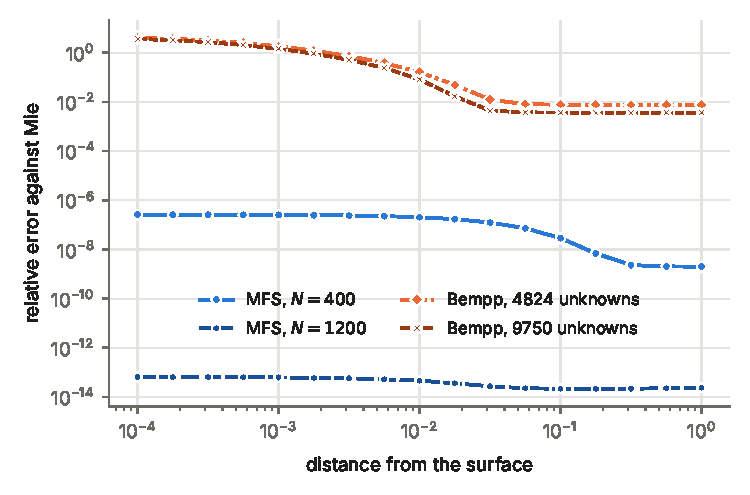
\includegraphics[width=0.68\textwidth]{fig_sphere_nearfield.pdf}
  \caption{Unit sphere, $k = 2\pi$: error of the scattered field against the Mie series as a function of the distance from the surface, for the MFS ($R_s = 0.5$) with $1200$ and $3600$ unknowns ($N = 400$ and $1200$ sources) and for Bempp with $4824$ and $9750$ unknowns (triangles of size $0.1$ and $0.07$, below which fixed-order quadrature loses accuracy).}
  \label{fig:nearfield}
\end{figure}

\subsection{The polyhedra and what the comparison shows}

On the cube, default quasi-uniform Bempp meshes still leave $2\times10^{-3}$ error after four minutes ($262$\,s), whereas edge-graded meshes are close at low accuracy (\autoref{tab:cubeends}, Figures~\ref{fig:cubecases} and~\ref{fig:costall}(d)). At the high-accuracy end, Bempp's largest mesh fitting in memory ($41472$ unknowns, $636\text{--}665$\,s) is overtaken by the MFS in $35\text{--}98$\,s ($14$\,s to $7.1\times10^{-5}$ at $k = 2\pi$ with one depth per octave), and the MFS continues past that $8$\,GB ceiling to $2.1\times10^{-5}$ in $83$\,s and $6.8\times10^{-6}$ in $123$\,s ($k = 2\pi$, standard wave). On the regular tetrahedron (\autoref{sec:tetrahedron}), the MFS envelope lies below symmetric graded Bempp at every accuracy, reaching $1.5\times10^{-3}$ in $4.4$\,s (versus $1.8\times10^{-3}$ in $6.8$\,s) and $1.0\times10^{-4}$ in $36$\,s (versus $2.2\times10^{-4}$ in $267$\,s). Near $10^{-3}$ on the cube, the MFS is faster for the standard wave at $k = 2\pi$ ($3.1$\,s versus $3.8$\,s), about $1.3\times$ for the general wave ($6.0$\,s versus $4.5$\,s), and twice as fast at $k = 4\pi$ and $6\pi$ ($6.3$\,s versus $12$\,s, and $15$\,s versus $34$\,s).

Between these two ends, the crossover moves towards coarser tolerances as frequency grows: from $4.0\times10^{-4}$ and $3.5\times10^{-4}$ (standard and general waves) at one wavelength to $8.0\times10^{-4}$ and $1.1\times10^{-3}$ at two and three wavelengths for two depths per octave alone, and to $9.8\times10^{-4}$, $7.7\times10^{-4}$, $3.7\times10^{-3}$ and $3.2\times10^{-3}$ once the fast one-depth variant is included ($1.3\times10^{-4}$ in $10.3$\,s against $86\text{--}149$\,s for Bempp at $k = 2\pi$).

\begin{table}[htbp]
  \centering
  \caption{Unit cube, both ends of the comparison. Left: the most accurate run of Bempp (on the $41472$-unknown mesh) and the first MFS run with a smaller error, each with its wall time. Right: wall time of the fastest run of each code with an error of about $10^{-3}$ (at most $1.2\times10^{-3}$; for the MFS, the faster of one and two depths per octave is taken).}
  \label{tab:cubeends}
  \small
  \setlength{\tabcolsep}{4pt}
  \begin{tabular}{llrlrrr}
    \toprule
     & \multicolumn{2}{c}{Bempp, most accurate} & \multicolumn{2}{c}{MFS, first better} & \multicolumn{2}{c}{Time [s] for $10^{-3}$} \\
    \cmidrule(lr){2-3}\cmidrule(lr){4-5}\cmidrule(lr){6-7}
    Case & Error & [s] & Error & [s] & Bempp & MFS \\
    \midrule
\tablebody{cube_ends}
    \bottomrule
  \end{tabular}
\end{table}

Overall, the MFS is faster across the tested range on smooth bodies and the regular tetrahedron, below $10^{-2}$ on the almond ($1.19$ and $3.5$\,GHz), and below $8\times10^{-4}\text{--}4\times10^{-3}$ across all four cube cases. Above those coarse cube tolerances, graded Bempp is competitive or $1.3\text{--}2$ times faster (oblique wave), whereas below them the gap opens rapidly: Bempp's effective algebraic order $p$ in $\varepsilon\propto N_u^{-p}$ drops from $1.4$ on coarse meshes to $0.8\text{--}1$ on fine ones, while that of the MFS rises from $2.7$ to $4.8$ (\autoref{fig:cubeconv}).

\section{Discussion and conclusion}
\label{sec:conclusion}

All five layouts follow from one principle: fictitious sources must enclose the singularities of the continued scattered field, or reach them where they meet $\Gamma$. Any non-resonant inner radius works on the sphere, whereas the focal ring bounds the torus surface from below, a focal curve runs within $6\%$ of the almond rim, and on the cube and tetrahedron the singular set meets $\Gamma$ along the edges and vertices of the skeleton. Wherever it touches $\Gamma$, singular tails with analytical wedge and conical exponents restore rapid convergence with few unknowns. We note two main limitations.

\emph{Generality and accuracy.} Each layout was built from the singular set of its geometry rather than generated automatically; \autoref{thm:skeleton} applies to convex conducting polyhedra only, while the torus bound \eqref{eq:torusradius} and almond focal curve rest on analytical heuristics and numerical tests rather than three-dimensional Maxwell proofs. Graded Bempp confirms the field to $6\times10^{-5}$ on the cube ($2\times10^{-4}$ on the regular tetrahedron and $1.2\times10^{-3}$ without symmetry on the asymmetric one, where fewer unknowns fit in $8$\,GB); beyond that, self-convergence places our cube reference error near $5\times10^{-6}$, with a fixed-$q$ floor further down.

\emph{Electrical size and comparison.} All bodies here are at most nine wavelengths long, dense factorisation scales cubically, and our timings compare against a lowest-order dense boundary element solver rather than a high-order or fast-multipole code. Because the skeleton columns separate into a coarse interior core and distinct edge walls with moderate condition numbers (below $3\times10^7$, \autoref{sec:method}), however, iterative least squares works without forming $A$. Orthogonalising each edge wall against the coarse core (inner points, vertex rays and two coarsest levels) stores $11\text{--}14$ times less memory than $A$ and converges to relative normal-equation residual $10^{-4}$ in $17\text{--}22$ matrix-free panel-tree LSMR \cite{fong2011} iterations on the cube ($J = 4,6,8$ at $k = 2\pi$ and $J = 6$ at $k = 4\pi$; $7\text{--}53$\,MiB versus $88\text{--}625$\,MiB) and $33\text{--}35$ on the asymmetric tetrahedron ($J = 4,5$; $158\text{--}259$\,MiB versus $2.10\text{--}3.51$\,GiB), matching direct solves to $1\text{--}6\times10^{-4}$ (whereas $54\text{--}100$ diagonal-scaled iterations leave $3\times10^{-3}\text{--}6\times10^{-2}$); fast multipoles would speed each product. Adding four and twelve modes per unit length handles $k = 4\pi$ and $6\pi$ (\autoref{sec:cubeother}), and a preliminary $k = 8\pi$ test reaches $10^{-3}$ with $24$ extra modes and five nodes per panel (six for finer levels).

In conclusion, on convex polyhedra and the NASA almond, the Maxwell MFS in three dimensions converges once sources sit on an interior set reaching the surface singularities, cluster towards its boundary contact, and continue below cut-off via parameter-free singular tails. With these layouts, root-exponential convergence holds down to $2\times10^{-5}$ on the cube and $10^{-4}$ on the regular tetrahedron (and without symmetry on an asymmetric one), and the NASA almond radar cross-section matches a published reference within $0.12$\,dB on average up to $10.25$\,GHz. Automating layout construction for general geometries is the natural next step.




\section*{Code and data availability}
The complete source code, including the scripts that generate every table and figure, is publicly available at \url{https://github.com/sap6/MFS}. The measured and simulated almond data are those of the Austin RCS Benchmark Suite \cite{kelley2020}.

%% TODO (authors): acknowledgements; declaration on the use of AI tools as
%% required by the journal (see NOTES.md, section 6).

\setlength{\bibsep}{1.5pt plus 0.5pt}
\bibliographystyle{elsarticle-num}
\bibliography{refs}

\end{document}
